\documentclass{article}
\usepackage{graphicx} % Required for inserting images

\title{Advancements in Aspect Extraction for Aspect-Based Sentiment Analysis}
\author{Prabesh Tandukar - Master of Software Engineering - Yoobee College}
\date{19 January 2024}

\begin{document}

\maketitle

\tableofcontents
\listoffigures
\listoftables

\newpage

\begin{abstract}
Aspect-based sentiment Analysis (ABSA) is an advanced branch of sentiment analysis that concentrates on identifying and evaluating sentiments related to specific aspects in a piece of text. This paper reviews various methods and models for effective aspect extraction in ABSA, such as Mutual Information Maximization, Shared Multitask Learning Network (SMLN), and Artificial Bee Colony (BeeAE). It also examines the performance of these methods against traditional and BERT-based modules, highlighting the superiority of the proposed techniques in accuracy and Micro-F1 scores. The paper further explores the applications of ABSA in real-world scenarios, addressing the challenges and potential future developments in the field. ABSA's significance is underscored by its ability to provide nuanced insights into consumer opinions, which is invaluable for businesses and organizations across various domains.
\end{abstract}

\section{Introduction}
The recent surge in social media usage has sparked an increased interest in the research field of Sentiment Analysis (SA) and Opinion mining. SA involves collecting, analyzing, and aggregating online content from different sources like social media platforms, blogs, e-commerce sites, movie review platforms, and many more. Nowadays, consumers tend to opt for products or services that have good reviews posted by others. However, going through each review can be very cumbersome so the need for opinion mining to enhance effective decision-making for individuals as well as organizations has developed.\cite{ansari2020aspect} 

Aspect-based sentiment Analysis (ABSA) is an essential component in sentiment analysis due to its ability to provide a detailed analysis of sentiments, focusing on specific aspects or features of a product, service, or topic rather than just an overall sentiment score. It considers the context of the sentiment, which is crucial for understanding the true meaning behind a statement. ABSA has wide-ranging applications across various domains, such as analyzing social media posts during critical events or in e-commerce. It can also be used to boost the results of machine learning models, for instance through data augmentation techniques. Furthermore, ABSA can be extended to multi-modal data, combining text with other data types like images, to provide a more comprehensive sentiment analysis\cite{Jiang2023AspectBasedSA}\cite{Gomes2023GABSAPTGN} \cite{lvarezLpez2018APF} \cite{Bensoltane2021ComparingWE} \cite{zhao2023m2df}. Figure 1 illustrates the structure related to the primary stages of ASBA.

\begin{figure}
    \centering
    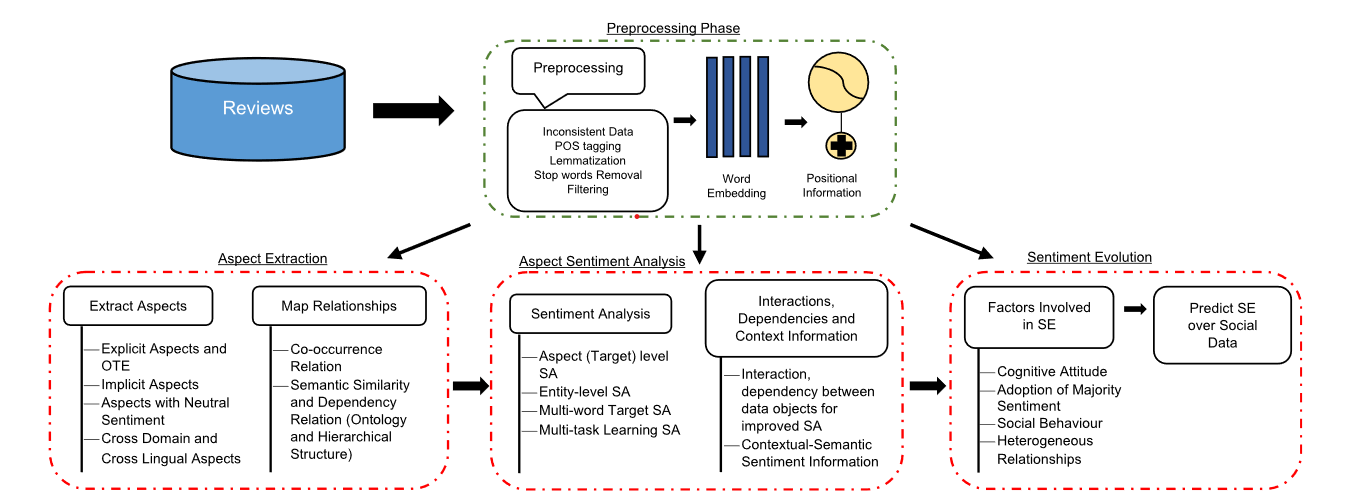
\includegraphics[width=1\linewidth]{asba.png}
    \caption{A framework of the main stages of aspect-based sentiment analysis}
    \label{fig: ASBA process}
    \cite{NazirIssues&Chall2023}
\end{figure}


\subsection{Research Questions: }
The literature review seeks to explore the following research questions:
\begin{enumerate}
  \item Identify Effective Methods for Aspect Extraction.
  \item Explore different Sentiment Analysis Techniques including rule-based approaches, machine learning-based approaches, and deep learning-based approaches.
  \item Explore well-known datasets for Aspect-Based Sentiment Analysis
  \item Investigate Real-World Applications and Challenges in ABSA
  \item Explore the latest advancement in Aspect-based sentiment analysis.
  
\end{enumerate}

\section{Fundamentals of Sentiment Analysis: }
Sentiment analysis, also referred to as opinion mining, is a research area that focuses on interpreting people's sentiments, attitudes, or emotions toward a certain subject\cite{NazirIssues&Chall2023}. The fundamental task in sentiment analysis is to identify the polarity of a given text, categorizing it as positive, negative, or neutral. This analysis can be conducted at various levels, such as document level, sentence level, or feature level.\cite{doi:10.1504/IJESMS.2021.119892}

\subsection{Challenges and Limitations of Traditional Sentiment Analysis: }    
Traditional sentiment analysis methods encounter numerous challenges, such as the inherent ambiguity of language, cultural influences, subtle linguistic distinctions, and the complexity of adapting text analysis solutions to various language vocabularies.\cite{doi:10.1504/IJESMS.2021.119892} 

\subsection{Need for Aspect-Based Sentiment Analysis:}
Aspect-based sentiment Analysis (ABSA) is a more detailed variant of sentiment analysis that focuses on extracting specific sentiment information from user-generated content. Its goal is to determine the sentiment polarities directed at particular aspect categories or entities mentioned within the text.\cite{Feng2022UnrestrictedAM} ABSA is particularly useful in situations where the sentiment expressed may be different for different aspects of a product or service. For example, a review may convey a positive sentiment about a product's cost but a negative sentiment about its quality. ABSA enables this level of detail in sentiment analysis, making it an essential tool for comprehending nuanced customer feedback.\cite{Feng2022UnrestrictedAM}

\section{Aspect-based Sentiment Analysis:}
Aspect-based sentiment Analysis is a sub-field of sentiment analysis that aims to extract detailed sentiment information from texts. Differing from general sentiment analysis, which usually assigns an overall sentiment rating to a text as positive, negative, or neutral, ABSA takes a more nuanced approach by pinpointing specific aspects or features mentioned in the text and assessing the sentiment directed towards each of these aspects.\cite{doi:10.1504/IJESMS.2021.119892} \cite{NazirIssues&Chall2023}

\subsection{Significance of ABSA:}
ABSA is particularly significant because it provides a more detailed understanding of sentiment in text. It allows for the extraction of nuanced sentiment information, which can be crucial in various applications such as product reviews, customer feedback analysis, and social media analysis. For instance, in a product review, a customer might express positive sentiment about the product's design but negative sentiment about its price. ABSA can identify these distinct sentiments towards different aspects of the product, providing valuable insights for businesses, marketers, and decision-makers. \cite{doi:10.1504/IJESMS.2021.119892}\cite{Jiang2023AspectBasedSA}

\subsection{Key Components of ABSA:}
The key components of ABSA include aspects, opinions, and sentiment polarity:
\begin{itemize}
  \item \textbf{Aspects}: These are the specific entities or features within the text that the sentiment is expressed towards. Aspects in a text can be either explicit or implicit. Explicit aspects are those that are directly stated in the text, while implicit aspects are those that are deduced from the context of the text.\cite{hua2023systematic} \cite{NazirIssues&Chall2023}
  \item \textbf{Opinions}: These are the subjective statements or expressions in the text that convey sentiment. Opinions can express various types of sentiment, including emotions, evaluations, appraisals, and speculations.\cite{hua2023systematic}
  \item \textbf{Sentiment Polarity}: This refers to the direction of the sentiment conveyed in the opinion, which can be categorized as positive, negative, or neutral.\cite{hua2023systematic}\cite{NazirIssues&Chall2023}
\end{itemize}

\subsection{Examples of ABSA: }
Consider the following review for a smartphone: \textit{"The phone has an excellent camera but the battery life is disappointing."} In this case, ABSA would identify \textit{"camera"} and \textit{"battery life"} as the aspects. The opinion about the camera is \textit{"excellent"}, which has a positive sentiment polarity. The opinion about the battery life is \textit{"disappointing"}, which has a negative sentiment polarity. Thus, ABSA provides a more granular analysis of the sentiment in the review, identifying distinct sentiments towards different aspects of the product.\cite{hua2023systematic}

\section{RQ 1: Identify Effective Methods for Aspect Extractions: }

Aspect extraction is a vital step in Aspect-Based Sentiment Analysis (ABSA), and recent studies have introduced several efficient techniques for this purpose:

\subsection{Mutual Information Maximization: }
This technique is used for unsupervised domain-adaptive Aspect-Based Sentiment Analysis (ABSA) and Aspect Term Extraction (ATE). It is based on the concept of maximizing the mutual information between different variables, which in this case are the aspects and sentiments in a sentence. The approach can serve as an additional enhancement to any model for cross-domain ABSA and ATE. It has demonstrated superior performance over leading methods in cross-domain ABSA, improving Micro-F1 scores by an average of 4.32\% across 10 different domain segments \cite{chen2022simple} as shown in Figure 2.
\begin{figure}
    \centering
    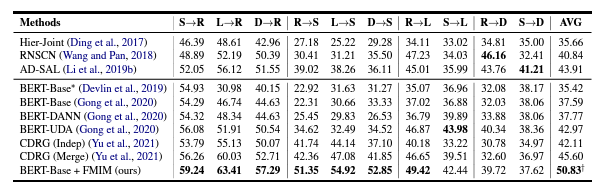
\includegraphics[width=1\linewidth]{MutualInformationMaximization.png}
    \caption{The Micro-F1 results for the Aspect Term Extraction (ATE) sub-task indicate that the performance of this study significantly surpasses that of the CDRG (Merge) method, as determined by a t-test.} 
    \label{fig:enter-label}
    \cite{chen2022simple}
\end{figure}

\subsection{Shared Multitask Learning Network (SMLN): }
This approach involves the training of related auxiliary tasks that are integral to aspect-level sentiment analysis \cite{Yao2021MultitaskLF}. It employs the 
 extraction of opinion terms due to their strong correlation with the primary task \cite{Yao2021MultitaskLF}. A specially designed Cross Interaction Unit (CIU) is used to transfer valuable information from the opinion term extraction task to the main task, thereby enhancing the performance of both tasks \cite{Yao2021MultitaskLF}. Figure 3 shows the SMLN framework.

As depicted in Table 1, the performance of the SMLN model is evaluated against traditional neural network methods, prior multitask learning methods, and other models that utilize the BERT representation \cite{Yao2021MultitaskLF}. The SMLN model demonstrates a notable enhancement in performance over the baseline methods on three datasets from SemEval-2014 and SemEval-2015 \cite{Yao2021MultitaskLF}. This enhancement is credited to the multitask learning setting and the information exchange mechanism in CIU module \cite{Yao2021MultitaskLF}.
\begin{figure}
    \centering
    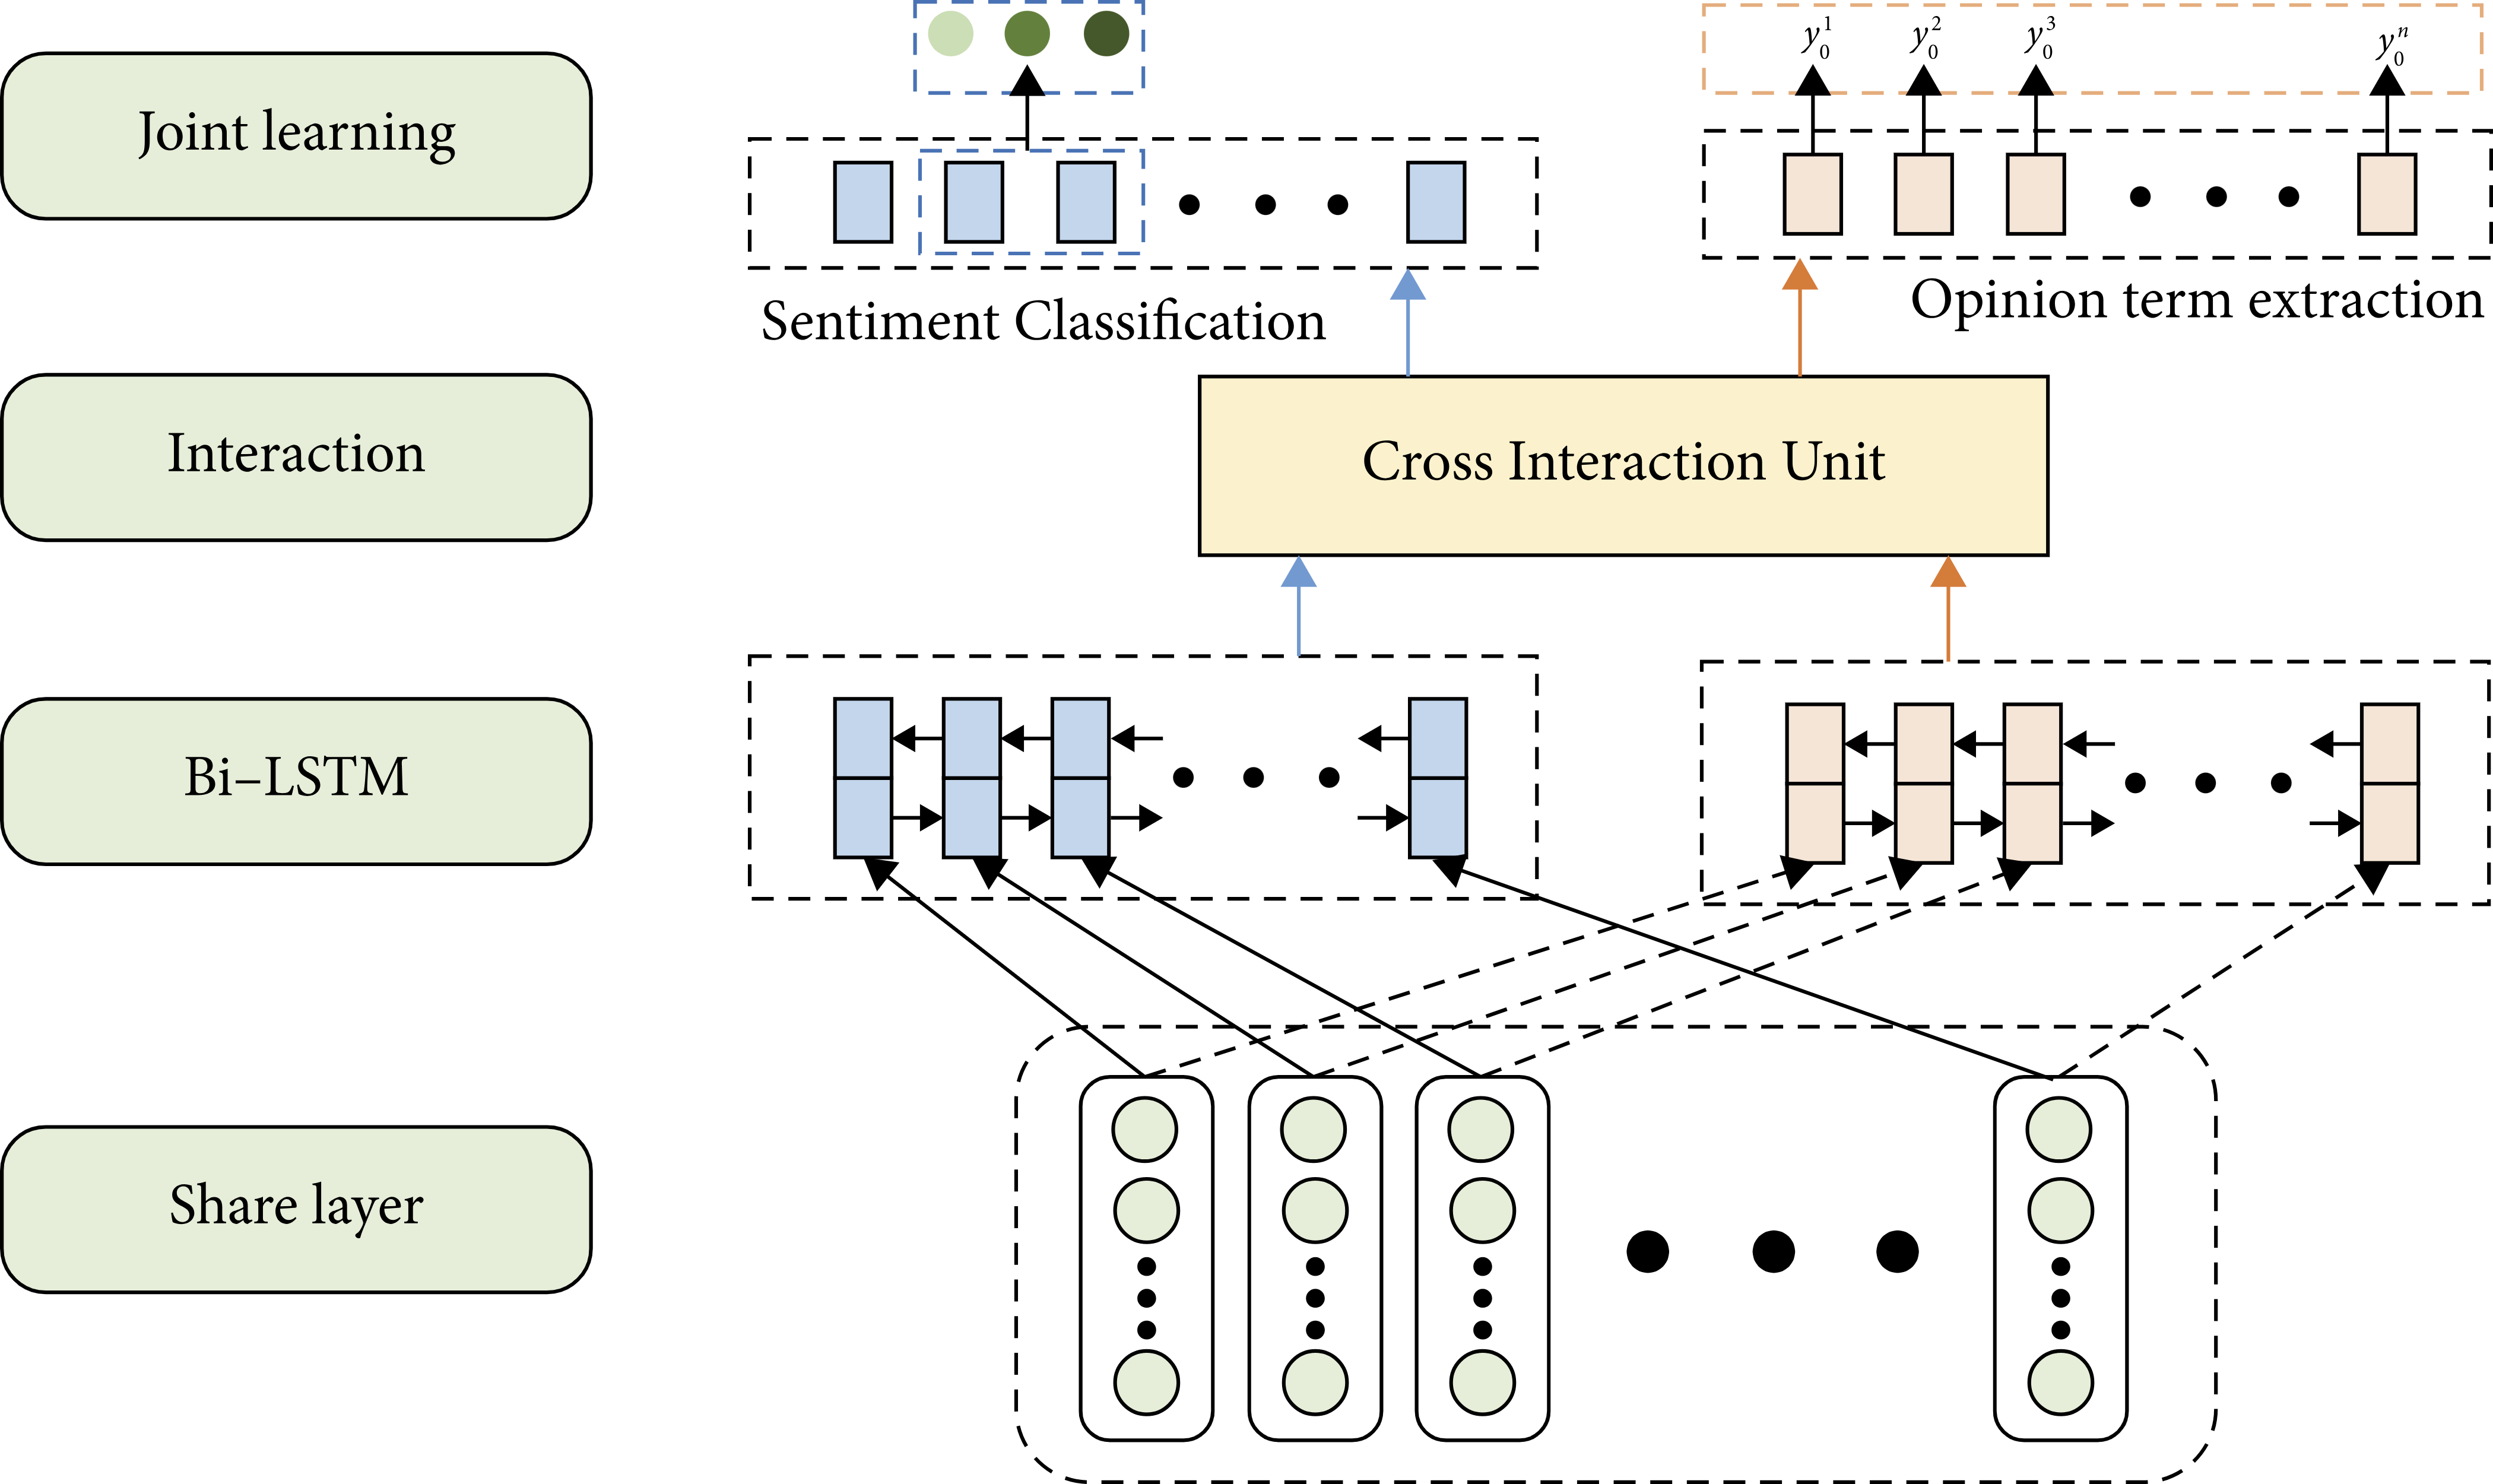
\includegraphics[width=0.5\linewidth]{SMLN.png}
    \caption{Framework of the proposed SMLN}
    \label{SMLN}
    \cite{Yao2021MultitaskLF}
\end{figure}

\begin{table}[h]
\centering
\begin{tabular}{|l|l|l|l|l|}
\hline
Method & Model & 14Lap & 14Res & 15Res \\ \hline
Conventional network & TD-LSTM (2016) & 68.13 & 75.63 & 76.39 \\ \hline
Conventional network & ATAE-LSTM (2016) & 68.70 & 77.20 & 78.48 \\ \hline
Conventional network & MemNet (2016) & 70.33 & 78.16 & 77.31 \\ \hline
Conventional network & TNET (2016) & 74.65 & 80.05 & 78.47 \\ \hline
Conventional network & IAN (2017) & 72.10 & 78.60 & 78.58 \\ \hline
Conventional network & RAM (2017) & 74.49 & 80.23 & 79.98 \\ \hline
Conventional network & TG-SAN (2020) & 75.27 & 81.66 & — \\ \hline
Multitask learning & PRET + MULT (2018) & 71.15 & 79.11 & 81.30 \\ \hline
BERT & IMN (2019) & 75.36 & 83.89 & 85.64 \\ \hline
BERT & BERT-FC (2018) & 76.54 & 81.28 & 81.52 \\ \hline
BERT & BERT-pair-QA-M (2019) & 77.93 & 85.12 & 81.89 \\ \hline
BERT & AEN-BERT (2019) & 78.35 & 81.46 & — \\ \hline
BERT & BERT-PT (2019) & 78.07 & 84.95 & — \\ \hline
BERT & TD-BERT (2019) & 78.87 & 85.10 & — \\ \hline
BERT & SK-GCN-BERT (2020) & 79.00 & 83.48 & 83.20 \\ \hline
BERT & SPRN-BERT (2021) & 79.31 & 85.03 & 85.30 \\ \hline
Our model & SMLN & 80.09 & 85.67 & 86.31 \\ \hline
\end{tabular}
\caption{Performance comparison of SMLN model with previous models, with average accuracy as the evaluation metric}
\label{tab:my_label}
\cite{Yao2021MultitaskLF}
\end{table}

\subsection{Artificial Bee Colony (BeeAE): }
This presents a new framework for extracting aspect terms that emphasize context features produced by pre-trained models. The process consists of four main steps. Initially, a collection of linguistic features linked to aspect terms is defined. Following that, the proposed feature selection artificial bee colony (FS-ABC) is utilized to pinpoint the features that are most relevant. This method tackles the issues of overlooking vital implicit linguistic features and not discovering enough valuable features for aspect term extraction \cite{Shi2022BeeAEEA}. An overview of the BeeAE framework is illustrated in Figure 3.
\begin{figure}
    \centering
    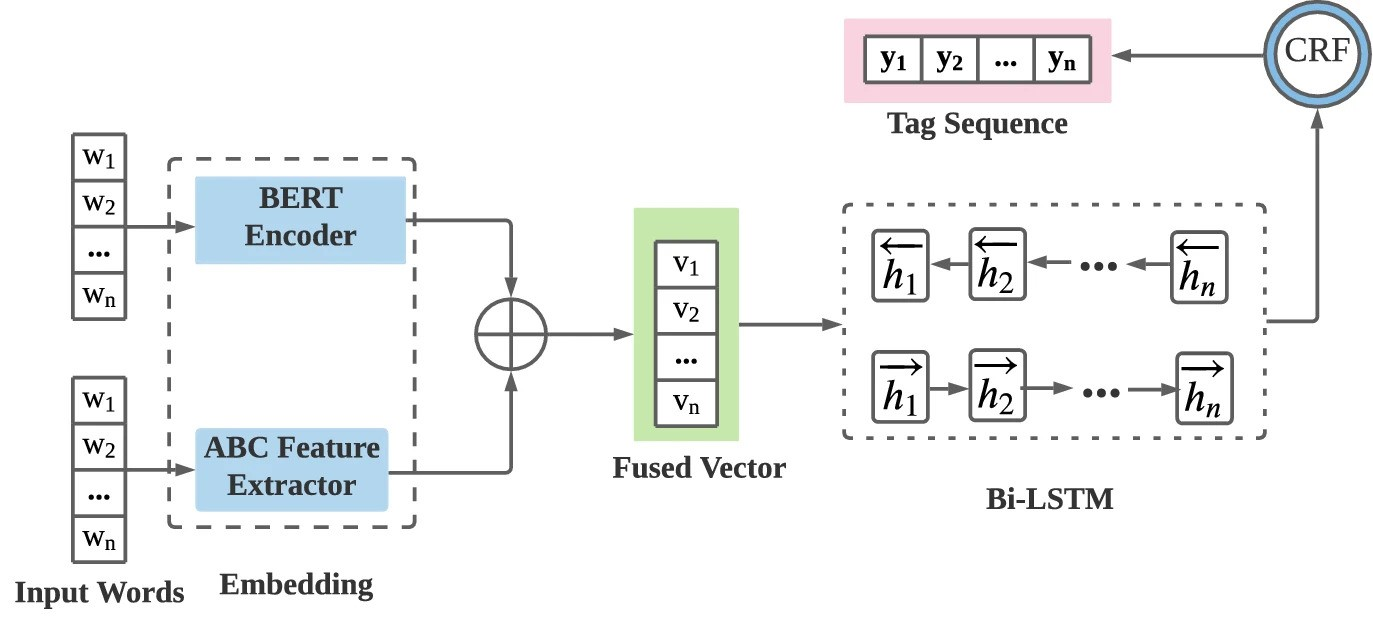
\includegraphics[width=0.5\linewidth]{BeeAE.jpg}
    \caption{The overview of the BeeAE framework.}
    \label{fig: BeeAE framework}
    \cite{Shi2022BeeAEEA}
\end{figure}

\section{RQ 2: Explore different Sentiment Analysis Techniques: }
ABSA employs a variety of techniques and models, including machine learning, natural language processing (NLP), and deep learning, to identify aspects and sentiments in text data. \cite{NazirIssues&Chall2023}

\subsection{Machine Learning Approaches: }
In ABSA, machine learning techniques are commonly employed to train models on annotated datasets to predict aspect sentiments in new, unseen texts. Widely used machine learning algorithms in ABSA include decision trees, random forests, logistic regression, and support vector machines (SVM).\cite{Adagale2023AspectBS}\cite{Horsa2023AspectBasedSA}. These algorithms have shown high accuracy in ABSA tasks with reported accuracy ranging from 85\% to 93\%.\cite{Horsa2023AspectBasedSA}\cite{hua2023systematic}

However, machine learning approaches have some limitations. These methods often require substantial volumes of annotated data for training, and their effectiveness can be influenced by the quality and representation of the training data. They may also struggle with implicit aspect extraction and complex relationships between opinions and aspects\cite{Adagale2023AspectBS}.

\subsection{Natural Language Processing Techniques:}
Natural Language Processing (NLP) techniques play a pivotal role in Aspect-Based Sentiment Analysis (ABSA) for tasks such as aspect extraction, sentiment classification, and opinion mining \cite{rocca2023natural}\cite{Adagale2023AspectBS}. These techniques can involve syntax-based methods, frequency-based methods, and feature extraction methods\cite{Adagale2023AspectBS}. For instance, Natural Language Processing (NLP) can be utilized to recognize named entities within a text (a process known as named entity recognition), to identify the primary themes present in a collection of texts (a process known as topic modeling), and to automatically determine the sentiment of a specific text (a process known as sentiment classification) \cite{rocca2023natural}

\subsection{Deep Learning Models: }
Deep learning models, a subset of machine learning models, have demonstrated encouraging outcomes in Aspect-Based Sentiment Analysis (ABSA). These models have the ability to autonomously learn to extract valuable features from raw text data, which can be advantageous for tasks such as aspect extraction and sentiment classification.\cite{Kumar2023AspectBasedSA} \cite{Dhanith2023ACE}

Some of the deep learning models used in ABSA include Convolutional Neural Networks (CNNs), Recurrent Neural Networks (RNNs), and Transformer-based models such as BERT (Bidirectional Encoder Representations from Transformers)\cite{Dhanith2023ACE}\cite{Kumar2023AspectBasedSA}. For example, a Sentiment-Support Graph Convolutional Network (SSGCN) has been proposed, which combines semantic and grammatical information to effectively analyze sentiment. \cite{Dhanith2023ACE}

Deep learning models can handle complex relationships in text data and can work well with large amounts of data. However, they can be computationally intensive and may require significant resources for training. They can also be more difficult to interpret compared to traditional machine learning models\cite{Kumar2023AspectBasedSA}\cite{Dhanith2023ACE}.

\subsection{Examples: }
Consider a review for a restaurant: \textit{"The food was delicious but the service was slow"}. A machine learning model trained for ASBA might identify \textit{"food"} and \textit{"service"} as the aspects, and \textit{"delicious"} and \textit{"slow"} as the opinions. It could then assign a positive sentiment to the aspect of food and a negative sentiment to the aspect of service. A deep learning model might perform a similar analysis but could potentially capture more nuanced sentiment information by considering the context and relationships between words in the review.


\section{RQ3: Popular Datasets for Aspect-Based Sentiment Analysis: }
Several datasets are commonly used for training and evaluating aspect-based sentiment analysis (ABSA) models. These datasets usually comprise of text data, such as reviews of products or posts on social media, annotated with aspects and their corresponding sentiments\cite{Dhanith2023ACE}\cite{hua2023systematic}.
\begin{itemize}
    \item \textbf{SemEval Datasets: } The SemEval (Semantic Evaluation) workshops have organized several tasks on ABSA, providing datasets in multiple languages and domains. These datasets are widely used in ABSA research\cite{hua2023systematic}\cite{NazirIssues&Chall2023}.
    \item \textbf{Multi-Aspect Multi-Sentiment (MAMS) Dataset: } This dataset stands out because each sentence includes at least two distinct aspects that carry different sentiments. It provides a challenging setting for ABSA models\cite{Dhanith2023ACE}.
\end{itemize}
However, these datasets have limitations. For instance, approximately 60\% of the aspects used for testing in widely used public datasets are not present in the training set\cite{hua2023systematic}. This means that many ASBA models are tested on aspects they have not seen during training, which can affect their performance.

\subsection{Evaluation Metrics for ABSA Models: }
The evaluation of ABSA models is commonly conducted using established machine learning metrics such as precision, recall, and the F1-score. These metrics are calculated for each aspect and sentiment and then averaged to provide an overall score\cite{hua2023systematic}\cite{NazirIssues&Chall2023}.
However, these metrics have limitations. For example, they do not account for the inherent complexity and variability of human language. They also do not consider the semantic similarity between predicted and actual aspects or sentiments, which can lead to overly harsh penalties for near-miss predictions\cite{NazirIssues&Chall2023}.

\subsection{Limitations of Existing Datasets and Evaluation Metrics: }
Existing datasets for ABSA have several limitations. They often lack diversity in aspects and sentiments, which can limit the generalizability of trained models. They also often contain imbalanced classes, with some aspects of sentiments being much more common than others. This can lead to models that perform well on common classes but poorly rare ones \cite{NazirIssues&Chall2023}.
Evaluation metrics for ABSA also have limitations. They often fail to capture the nuanced performance of models, especially when dealing with complex or implicit aspects and sentiments. They also do not account for the inherent subjectivity of sentiment analysis, where different individuals may have different interpretations of the same text \cite{NazirIssues&Chall2023}\cite{Dhanith2023ACE}.

\section{RQ 4: Real-World Applications of Aspect-based Sentiment Analysis: }
Aspect-based Sentiment Analysis (ABSA) has a wide range of applications in the real world, particularly in this business sector. It is used to analyze and understand people's opinions at the aspect level, which can provide more nuanced and detailed insights than traditional sentiment analysis \cite{hua2023systematic}.
\begin{itemize}
    \item \textbf{Customer Reviews: } ABSA is often used to analyze customer reviews. By identifying specific aspects and their associated sentiments, businesses can gain a deeper understanding of customer opinions. This can help them identify strengths and weaknesses in their products or services, and make informed decisions to improve customer satisfaction \cite{Horsa2023AspectBasedSA}
    \item \textbf{Social Media Analysis: } ABSA can also be used to analyze social media posts. This can provide insights into public opinion on various topics, helping businesses and other organizations to monitor their reputation, understand customer needs and preferences, and respond to emerging trends\cite{hua2023systematic}
\end{itemize}

\subsection{Challenges and Open Issues in ABSA: }
Despite its potential, ABSA faces several challenges and open issues: 
\begin{itemize}
    \item \textbf{Domain-Specific Nuances: } ABSA models often struggle to handle domain-specific nuances. For instance, a single word can convey varying sentiments depending on the context or domain it's used in. This makes it challenging to build ABSA models that can generalize well across different domains \cite{NazirIssues&Chall2023}\cite{doi:10.1504/IJESMS.2021.119892}.
    \item \textbf{Diverse Opinions: } Many texts, such as customer reviews or social media posts, contain diverse opinions towards different aspects. This makes it difficult to accurately identify and analyze all relevant aspects and their associated sentiments \cite{NazirIssues&Chall2023}.
    \item \textbf{Implicit Aspects: } ABSA models often struggle to handle implicit aspects, where the sentiment is expressed towards an aspect that is not explicitly mentioned in the text. This requires a deep comprehension of the text and its context, a task that poses a significant challenge for existing Aspect-Based Sentiment Analysis (ABSA) models \cite{NazirIssues&Chall2023}.
    \item \textbf{Cross-Lingual and Cross-Domain Challenges: } ABSA models often struggle to handle texts in different languages or from different domains. This is due to the scarcity of annotated data in numerous languages and domains, as well as the inherent differences in language use and sentiment expression across different languages and domains \cite{Verma2022ASO}.
    \item \textbf{Aspect and Sentiment Evolution: } The aspect that people care about and the sentiments they express can change over time. Current ABSA models often struggle to handle this dynamicity, which can affect their performance and usefulness in real-world applications\cite{NazirIssues&Chall2023}.
    
\end{itemize}

\section{RQ 5: Recent Advances And Trends: }

\subsection{Recent Research Papers and Advancements in ABSA: }
Several recent research papers and advancements have contributed to the field of Aspect-Based Sentiment Analysis (ABSA):

\begin{itemize}
    \item \textbf{Semi-supervised Model for Aspect Sentiment Detection: } This research introduced a semi-supervised model for Aspect-Based Sentiment Analysis (ABSA) tailored for online reviews, aiming to accurately predict both explicit and implicit sentiments across three domains: laptops, restaurants, and hotels. The proposed models surpassed earlier baseline models in terms of the F1-score for detecting aspect categories and the accuracy of sentiment detection\cite{Madhoushi2023SemiSupervisedMF}.

    \item \textbf{Meta-Based Self-Training and Re-Weighing for ABSA: } This research introduced a meta-based self-training method with a meta-weighter (MSM) to tackle challenges such as unbalanced labels and difficulties in sub-task learning in multi-task learning (MTL)-based Aspect-Based Sentiment Analysis (ABSA). The MSM method involves training a teacher model to generate in-domain knowledge. The pseudo-labels produced by this teacher model are then utilized by a student model for supervised learning\cite{He2023MetaBasedSA}.

    \item \textbf{OATS: Opinion Aspect Target Sentiment Quadruple Extraction Dataset for ABSA: } This paper presents the OATS dataset, which introduces three new domains and is comprised of 20,000 sentence-level quadruples and 13,000 review-level tuples. The OATS dataset is designed to address certain gaps in ABSA research, such as the repetitive emphasis on well-known domains like restaurants and laptops, the scarcity of data for complex quadruple extraction tasks, and the occasional neglect of the relationship between sentence and review-level sentiments\cite{chebolu2023oats}.

    \item \textbf{SENER: Sentiment Element Named Entity Recognition for ABSA: } This study introduced a concept known as Sentiment Element Named Entity Recognition (SENER) for Aspect-Based Sentiment Analysis (ABSA). SENER combines the principles of Named Entity Recognition (NER) and generative ABSA to identify sentiment entities using predefined sentiment element names. This approach enhances the understanding of both semantic and sentiment structures\cite{Lee2023SENERSE}.
\end{itemize}

\subsection{Advancements and Innovations Defining the Future of Aspect-Based Sentiment Analysis: }
Several advancements and innovations defining the future of Aspect-based Sentiment Analysis:
\begin{itemize}
    \item \textbf{Integration of Deep Learning Methods: } The integration of deep learning methods in ABSA is a significant trend. These methods automate the process of learning representations and are especially beneficial for identifying implicit sentiments when there is a limited amount of labeled data \cite{Madhoushi2023SemiSupervisedMF}.
    \item \textbf{Meta-Based Self-Training: } Meta-based self-training methods, such as the MSM proposed in recent research, are emerging as a promising approach to address issues in MTL-based ABSA. These methods create domain-specific knowledge and assign each instance with weights specific to the sub-task, which helps to manage their convergence rates, balance class labels, and mitigate the effects of noise introduced through self-training \cite{He2023MetaBasedSA}.
    \item \textbf{Development of New Datasets: } The development of new datasets, such as the OATS dataset, is another important trend. These datasets aim to address the limitations of current datasets and provide more comprehensive and diverse data for ABSA \cite{chebolu2023oats}.
    \item \textbf{Named Entity Recognition for ABSA: } The integration of named entity recognition (NER) in ABSA, as proposed in the SENER method, is an emerging trend. This method aids in identifying sentiment entities using predefined sentiment element names, which enhances the comprehension of semantic and sentiment structures\cite{Lee2023SENERSE}.
\end{itemize}


\section {Conclusion: }
The exploration of aspect extraction methods in Aspect-Based Sentiment Analysis has revealed significant advancement in the field. Techniques like Mutual Information Maximization and Shared Multitask Learning Networks have demonstrated their effectiveness by outperforming traditional models and enhancing cross-domain ABSA. The introduction of novel frameworks such as BeeAE has addressed the need for capturing implicit linguistic features and exploring valuable context features. The research indicated that ASBA is evolving rapidly, with new models and approaches continuously emerging to improve aspect extraction and sentiment analysis. Despite these advancements, challenges such as domain-specific nuances and diverse opinions remain. However, the potential of ABSA to revolutionize sentiment analysis in various applications is undeniable, making it a promising area for future research and development.

\bibliographystyle{plain} %choose your preferred bibliography style

\bibliography{mybibliography} %include your biblogrpahy file

\end{document}
